\section{Diagrama de Objetivos y Requerimientos}
\subsection{Diagrama general}
En este diagrama se muestra cuáles son los objetivos más grandes del proyecto, que se desarrollan en el resto de los diagramas.
\begin{figure}[H]
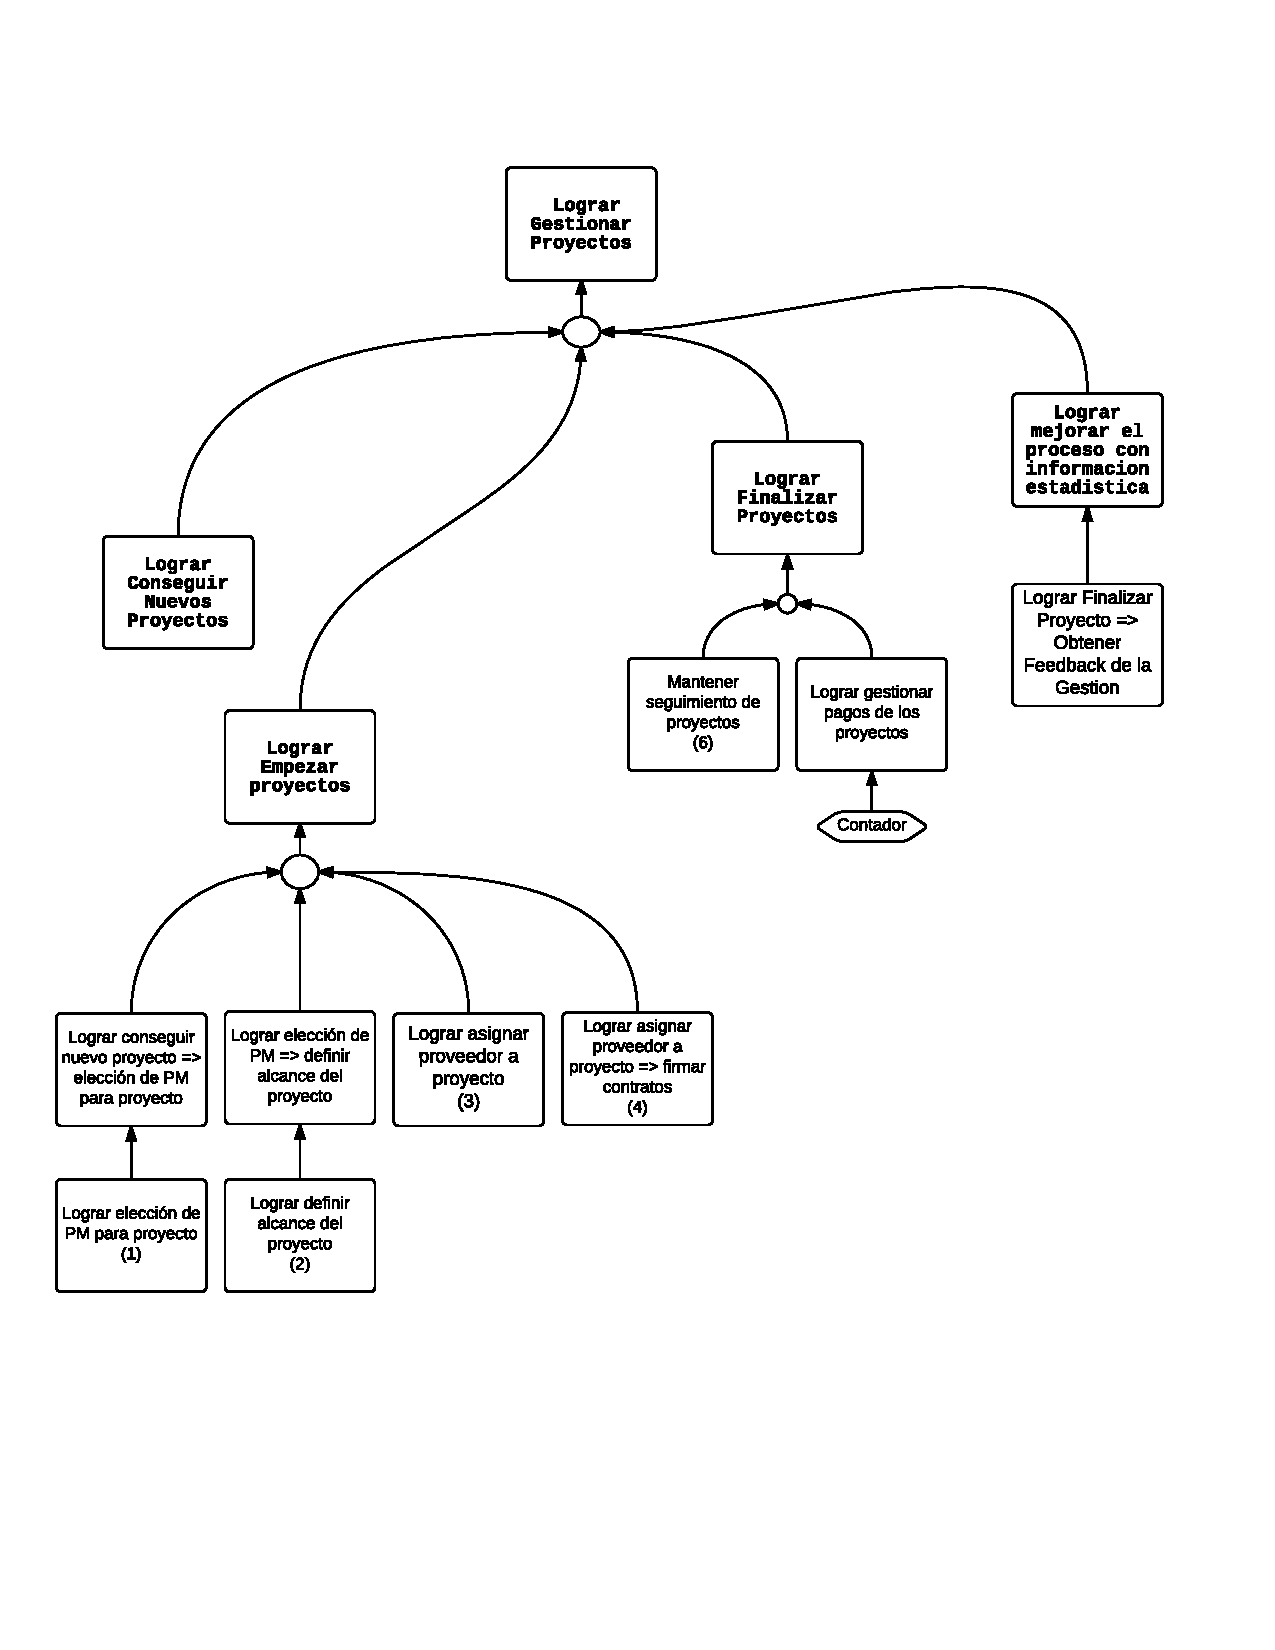
\includegraphics[width=\textwidth, clip=true, trim=15pt 170pt 15pt 80pt]{imagenes/objetivos/objetivos10.pdf}
\end{figure}
Podemos ver que los objetivos se dividen en los que permiten comenzar proyectos a partir de pre-proyectos, seguir proyectos en curso, conseguir nuevos proyectos (proveer herramientas para cargar preproyectos) y el circuito de feedback.

En particular el sistema de pagos no tiene que ver con el sistema, por lo tanto, no hay requerimientos de sistema que se vean en esta parte.

\subsection{Lograr Comenzar Nuevos Proyectos}
\begin{figure}[H]
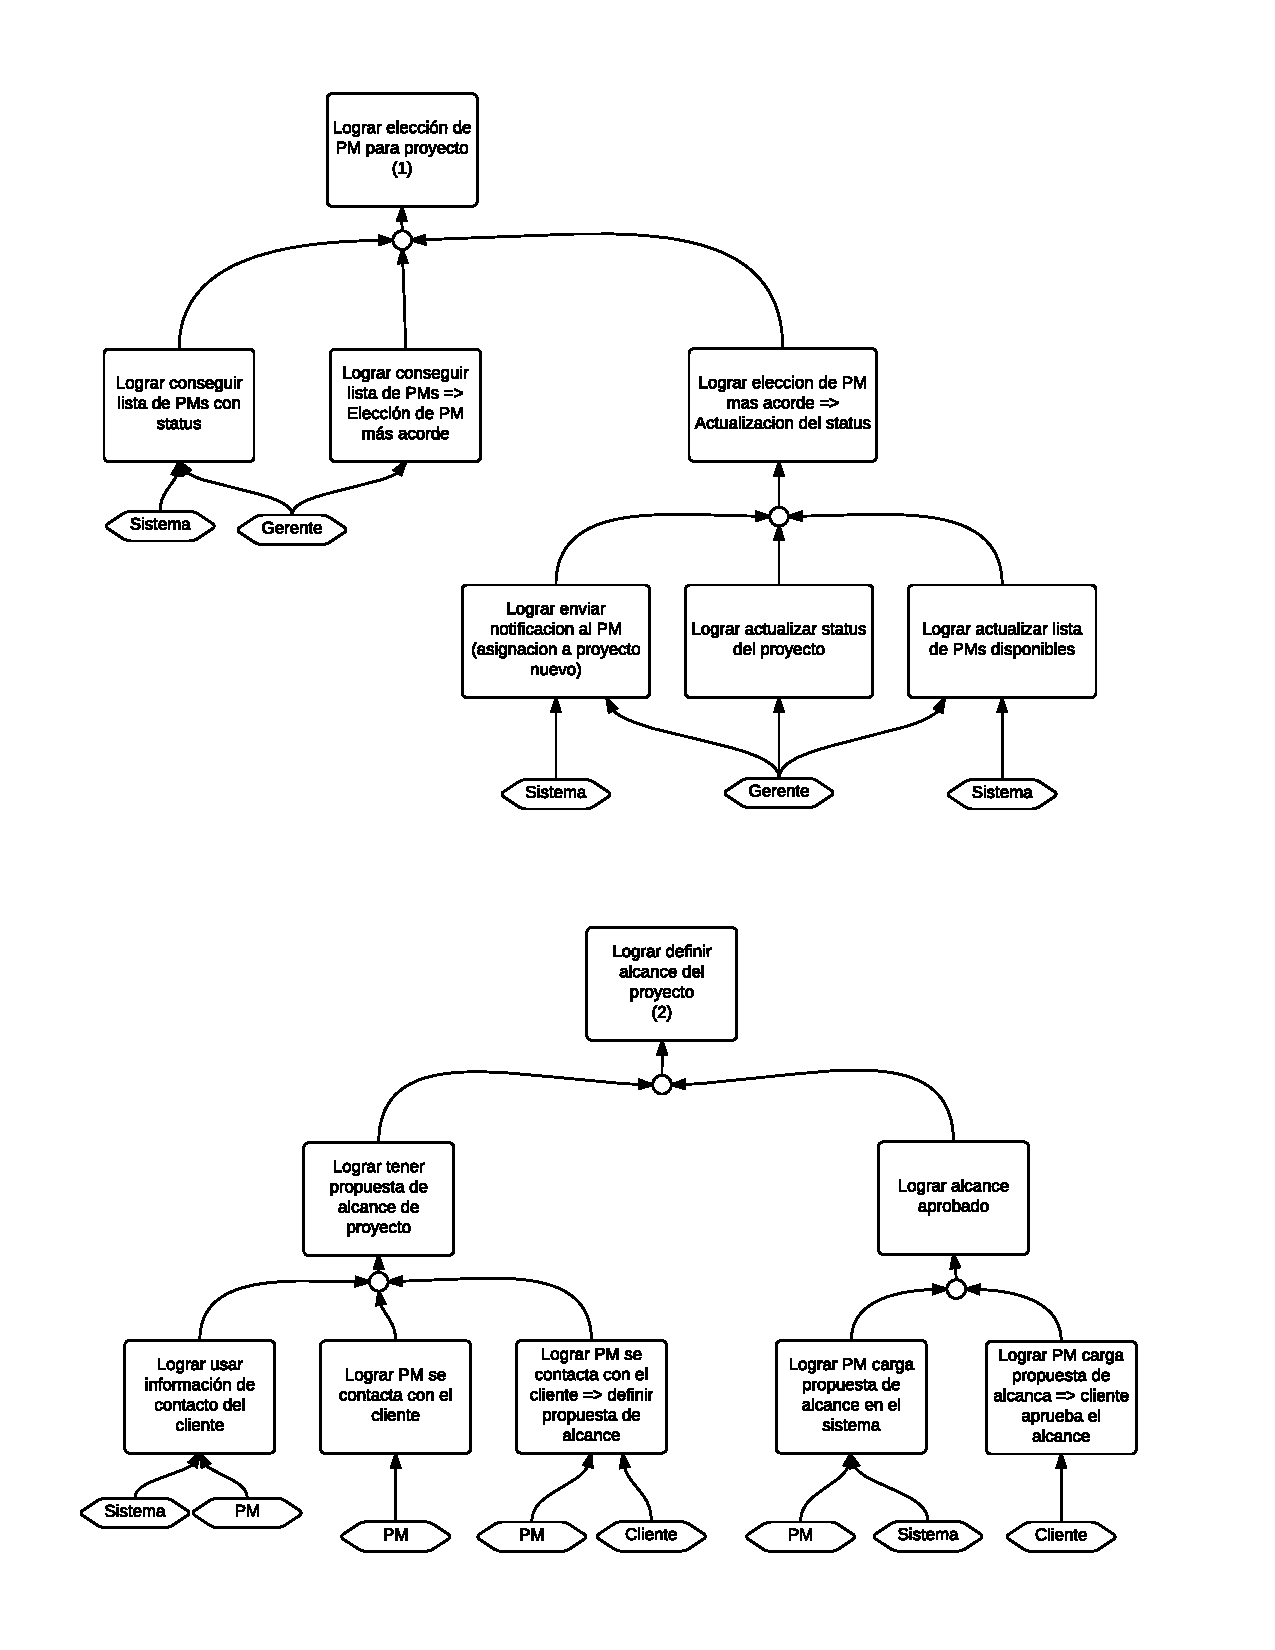
\includegraphics[width=\textwidth, clip=true, trim=15pt 0pt 15pt 0pt]{imagenes/objetivos/objetivos11.pdf}
\end{figure}
\begin{figure}[H]
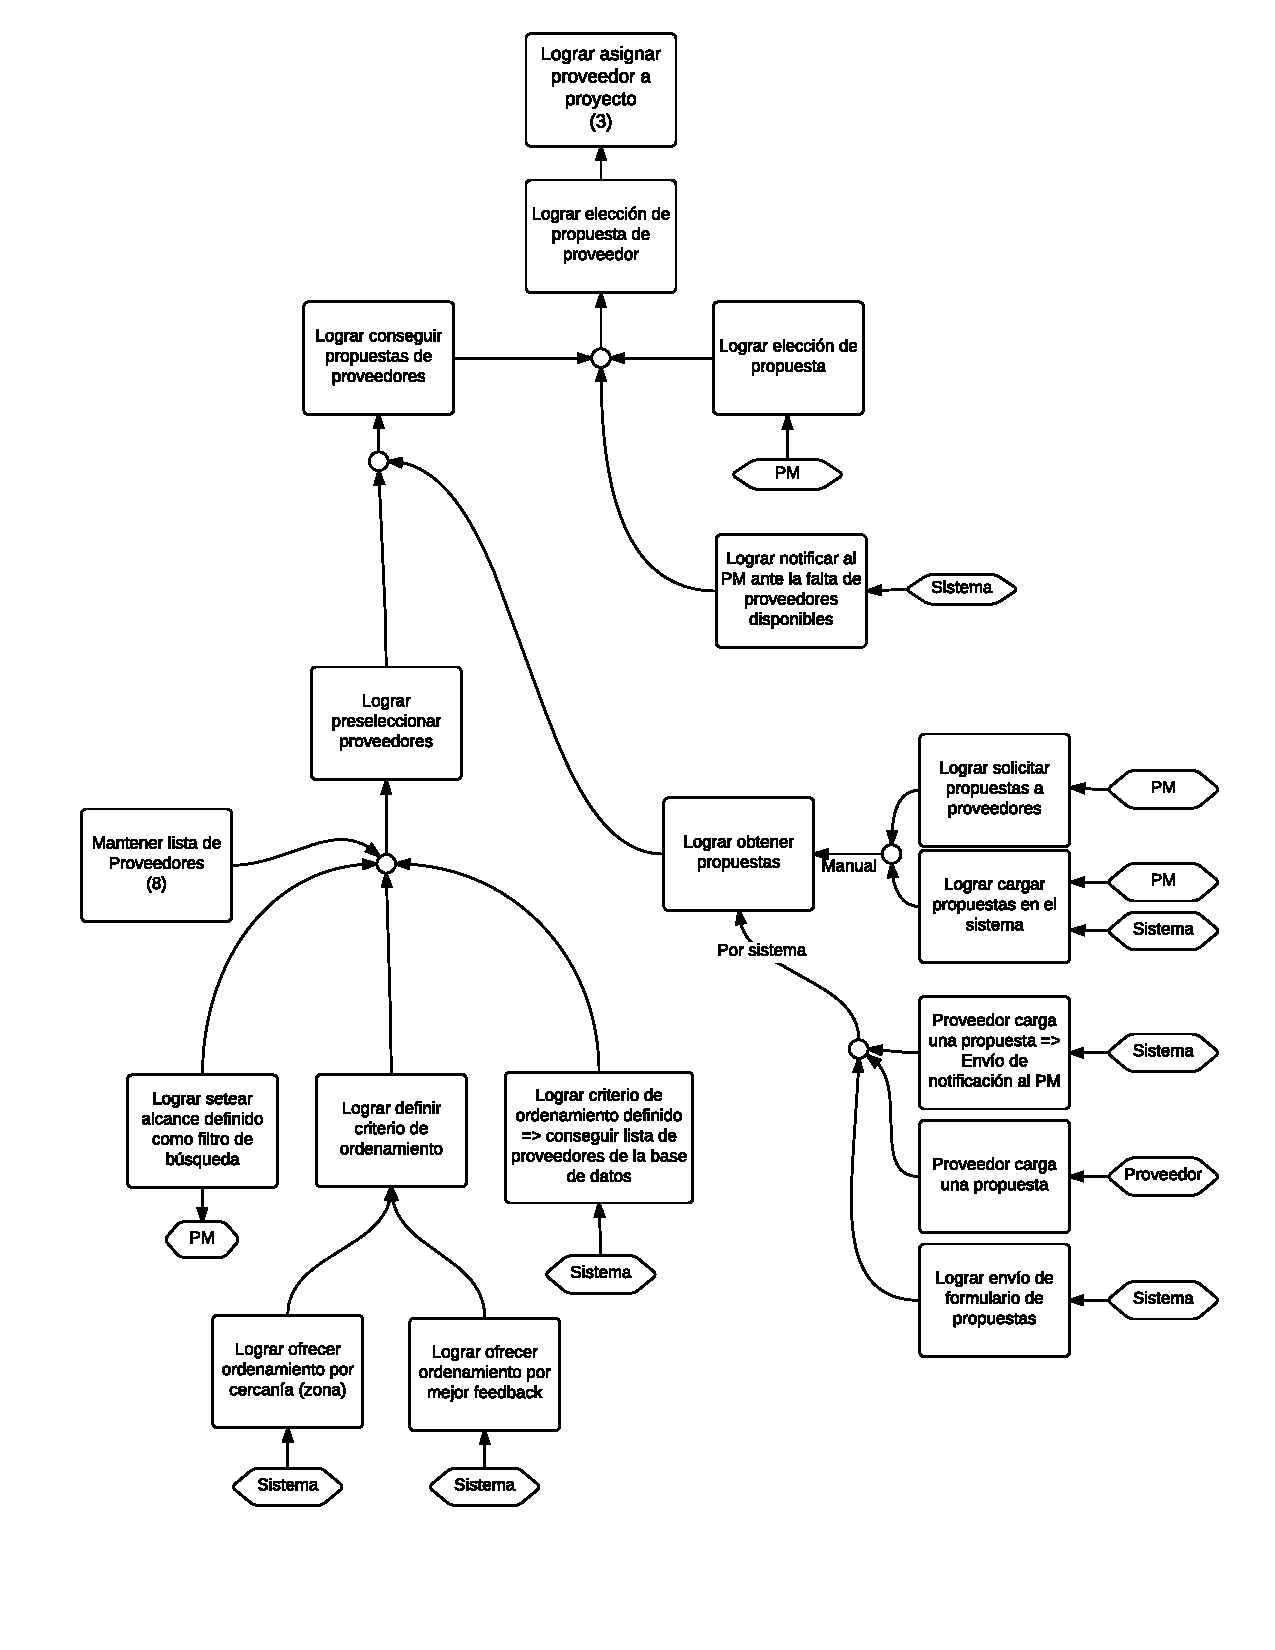
\includegraphics[width=\textwidth, clip=true, trim=15pt 0pt 15pt 0pt]{imagenes/objetivos/objetivos12.pdf}
\end{figure}
\begin{figure}[H]
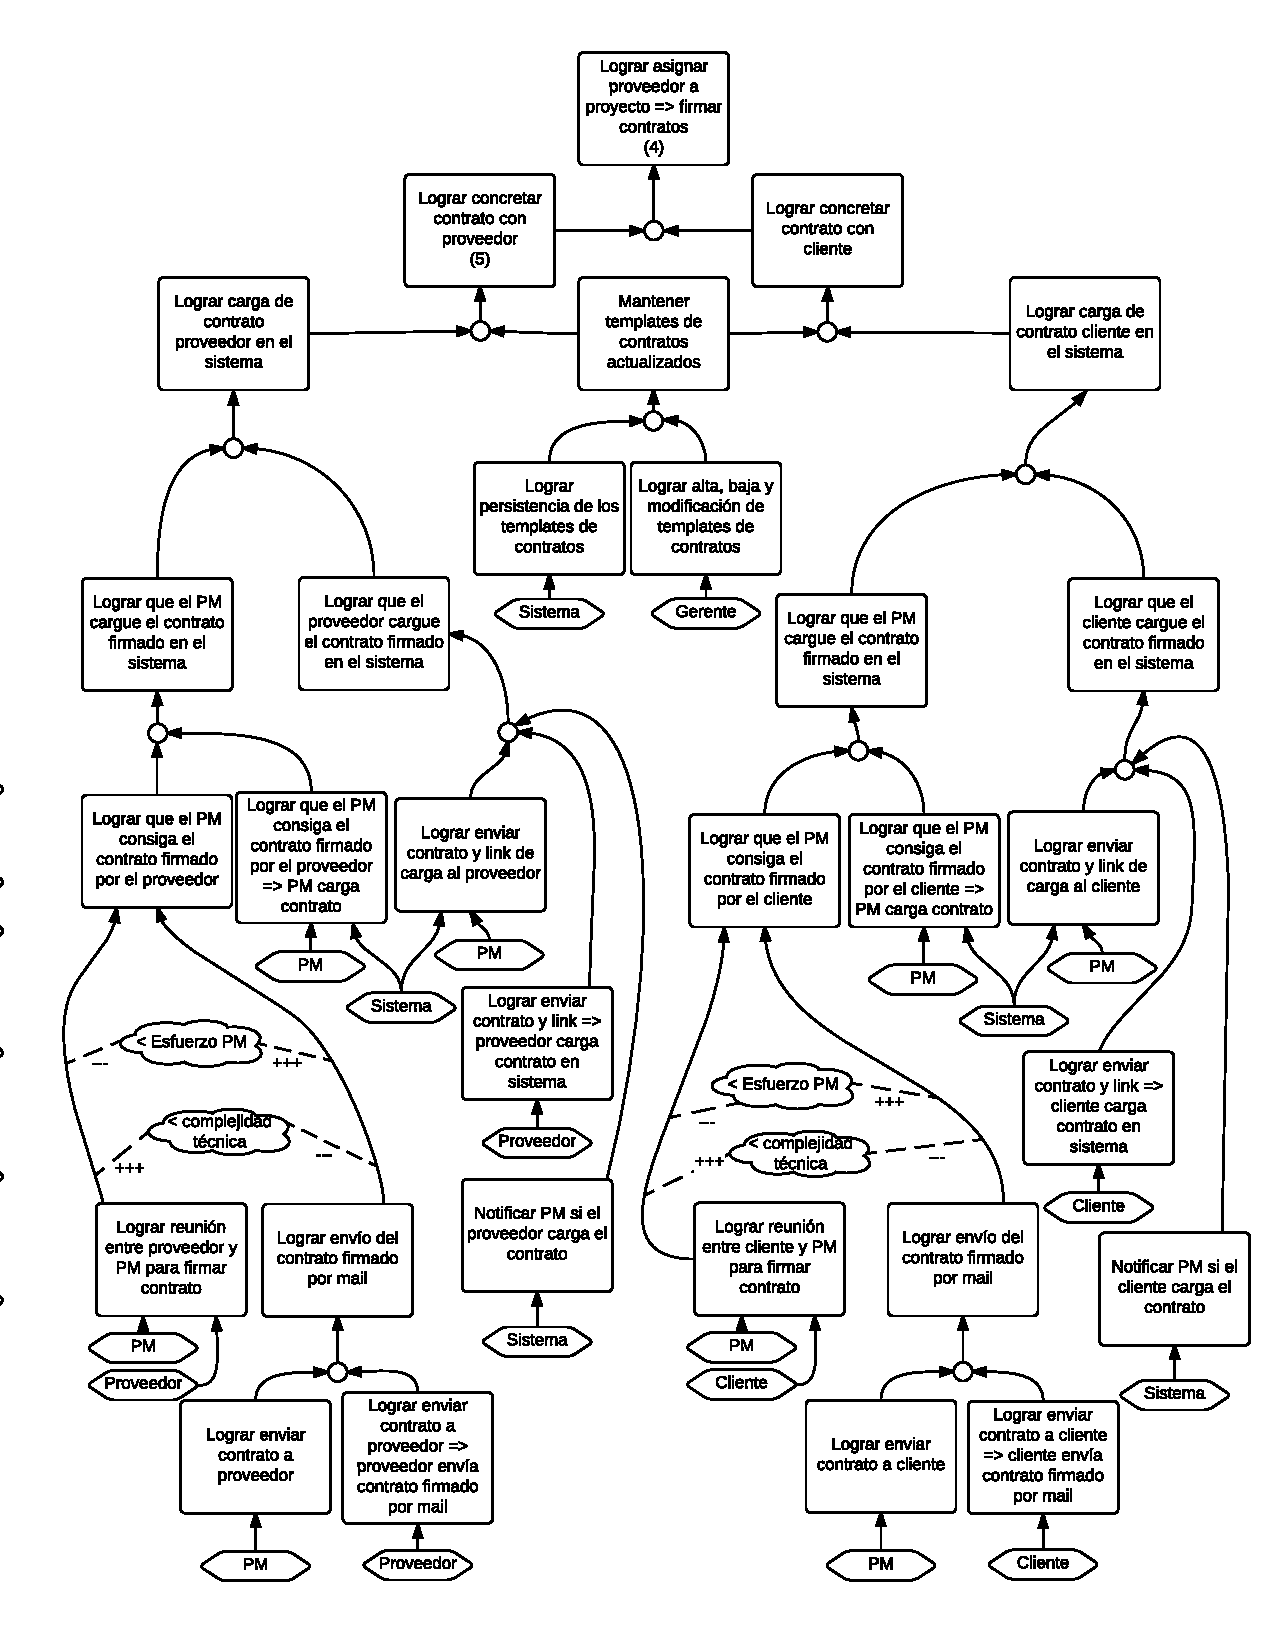
\includegraphics[width=\textwidth, clip=true, trim=15pt 0pt 15pt 0pt]{imagenes/objetivos/objetivos13.pdf}
\end{figure}

\newpage
\subsubsection{Requerimientos de Sistema}
Los requerimientos para esta parte son:
\begin{itemize}
	\item En la asignación de PM:
	\begin{itemize}
		\item Ofrecer una lista de PMs con sus status
		\item Permitir al gerente asignar un PM a un proyecto %FALTA EN DIAGRAMA
		\item Enviar notificaciones al PM al ser asignado a proyecto nuevo
		\item Actualizar lista de PMs disponibles
	\end{itemize}
	\item En la definición del alcance:
	\begin{itemize}
		\item Ofrecer información de contacto del cliente
		\item Ofrecer al PM cargar propuestas de alcance
	\end{itemize}
	\item En la asignación de proveedor:
	\begin{itemize}
		\item Dado un criterio de ordenamiento, ofrecer lista de proveedores más relevantes
		\item Implementar filtros por zona y por puntaje
		\item Notificar si no hay un proveedor disponible
		\item Notificar obtención de proveedor %SACAR?
		\item Ofrecer al PM cargar propuestas en sistema
		\item Ofrecer al proveedor cargar propuestas en sistema mediante link de carga
		\item Notificar al PM ante una carga de propuesta de un proveedor
	\end{itemize}
	\item En la firma de contratos:
	\begin{itemize}
		\item Almacenar y permitir al PM seleccionar templates para contratos.
		\item Proveer al PM mecanismos de carga de contratos (tanto para contratos de clientes como de proveedores).
		\item Proveer links de carga de contratos a proveedores y clientes
		\item Notificar al PM ante la carga de un contrato por parte de otro agente (cliente o proveedor). %AGREGAR
	\end{itemize}
\end{itemize}

\subsection{Seguimiento de Proyectos}
\begin{figure}[H]
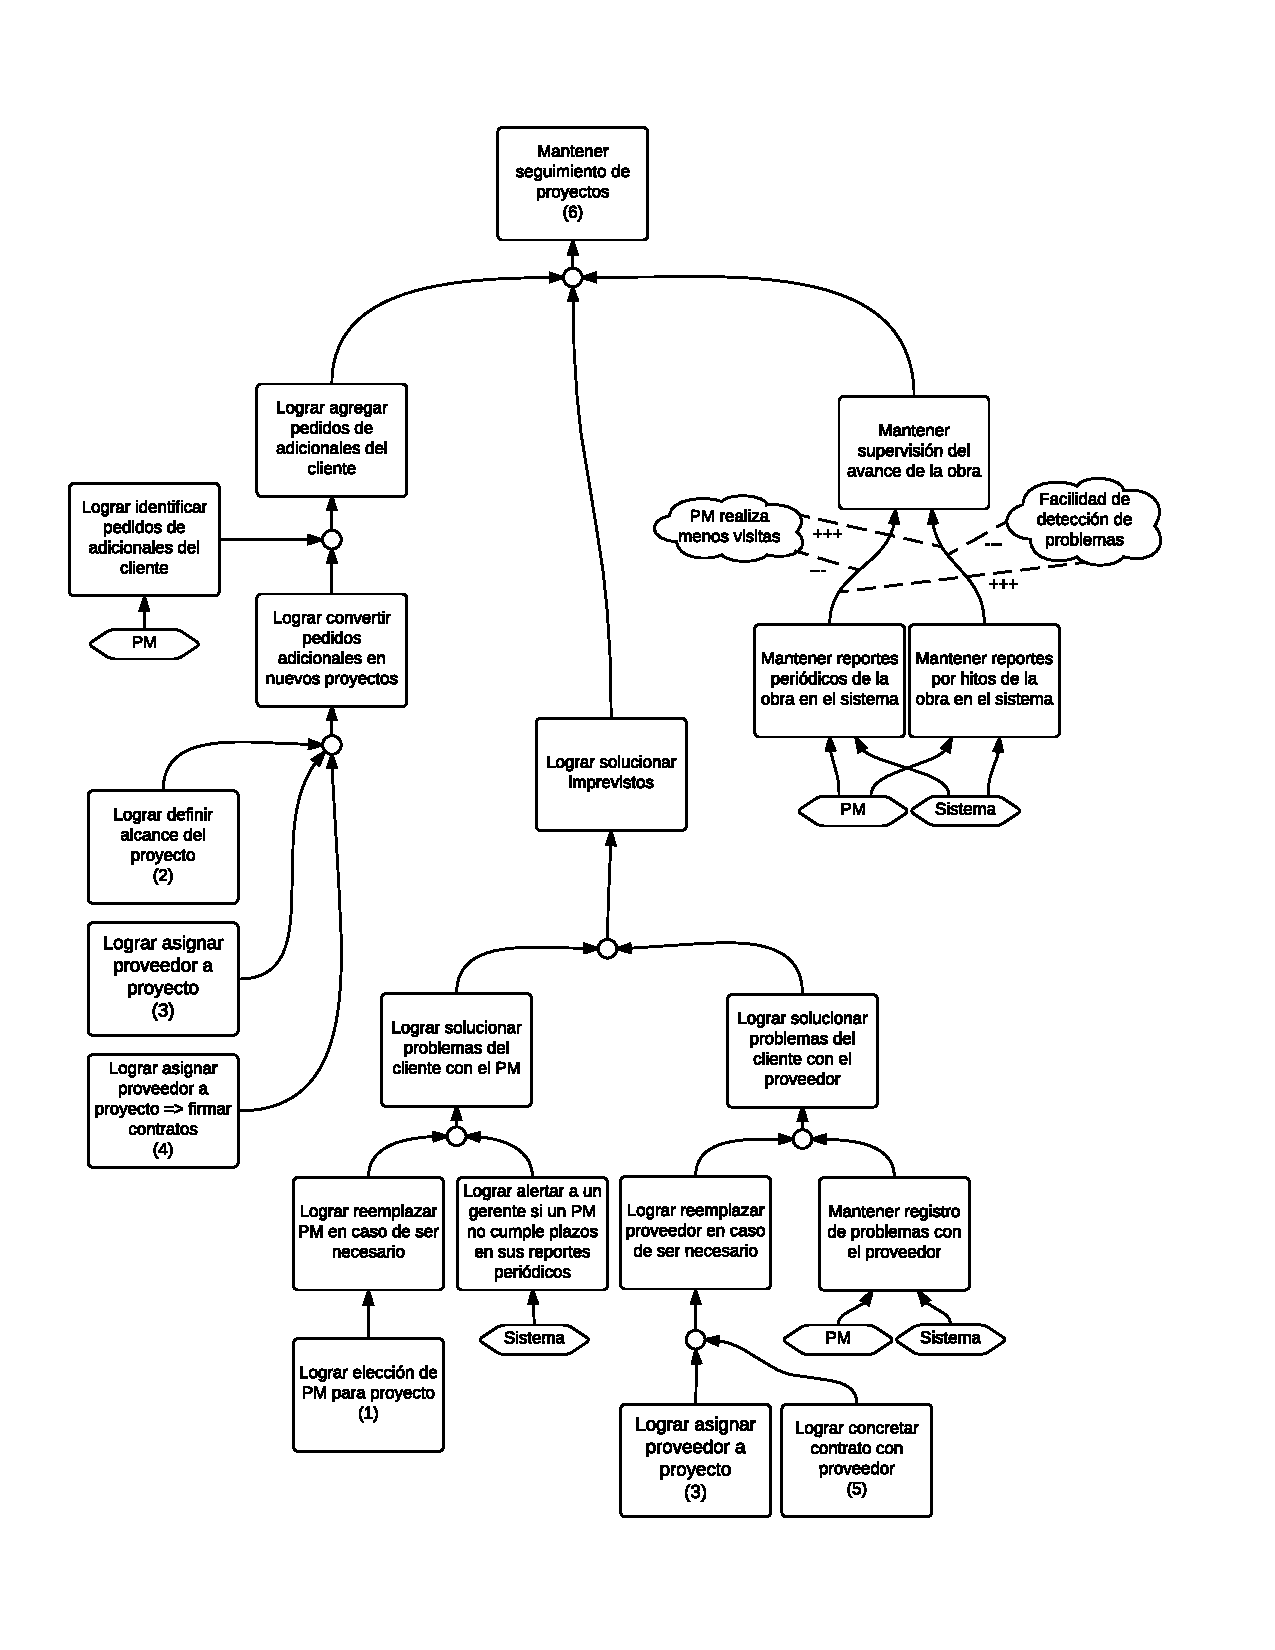
\includegraphics[width=\textwidth, clip=true, trim=15pt 50pt 15pt 60pt]{imagenes/objetivos/objetivos14.pdf}
\end{figure}

\subsubsection{Requerimientos de Sistema}
Los requerimientos para esta parte son:
\begin{itemize}
	\item Proveer interfaz al PM para cargar reportes de estado de proyectos.
	\item Alertar al gerente si un PM no carga sus reportes en los plazos establecidos.
	\item Mantener un registro de incidentes relacionados con el proveedor.
\end{itemize}

\subsection{Conseguir Nuevos Proyectos}
\begin{figure}[H]
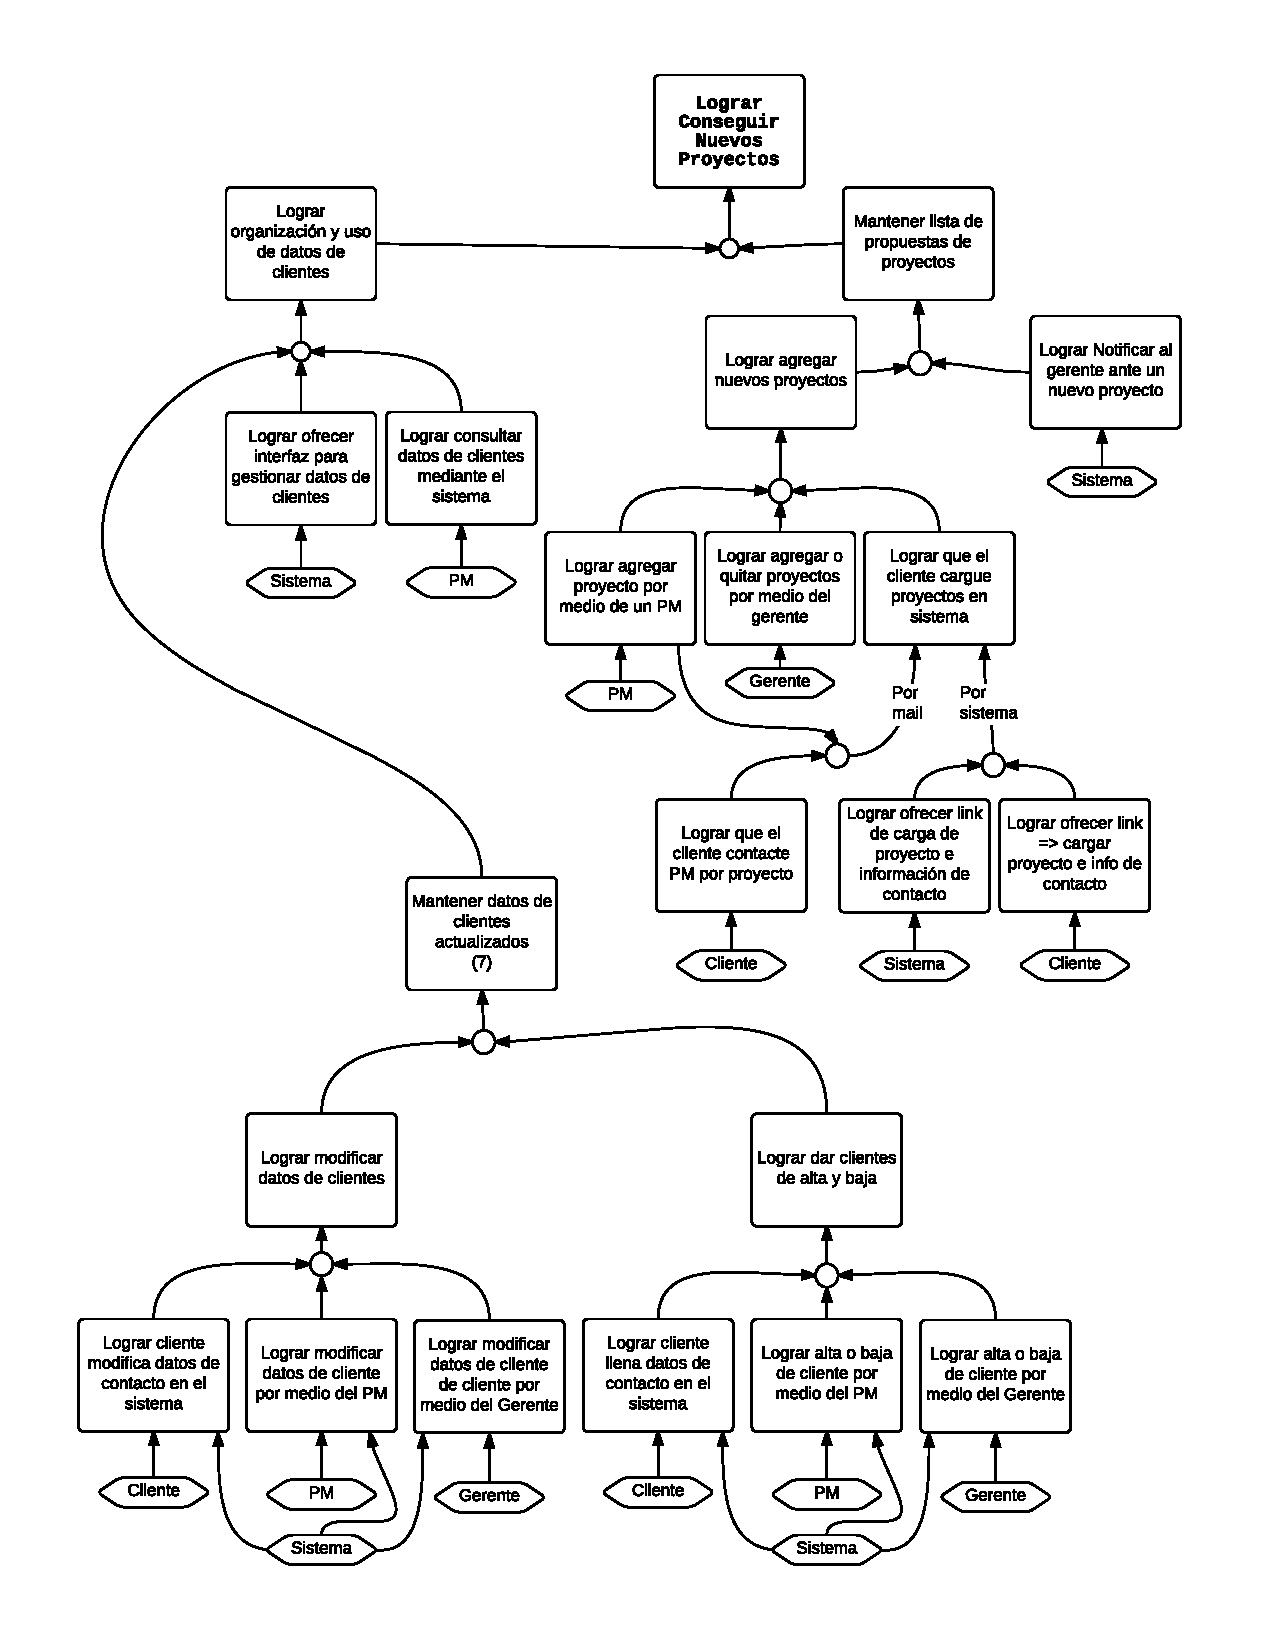
\includegraphics[width=\textwidth, clip=true, trim=15pt 20pt 15pt 20pt]{imagenes/objetivos/objetivos15.pdf}
\end{figure}
\begin{figure}[H]
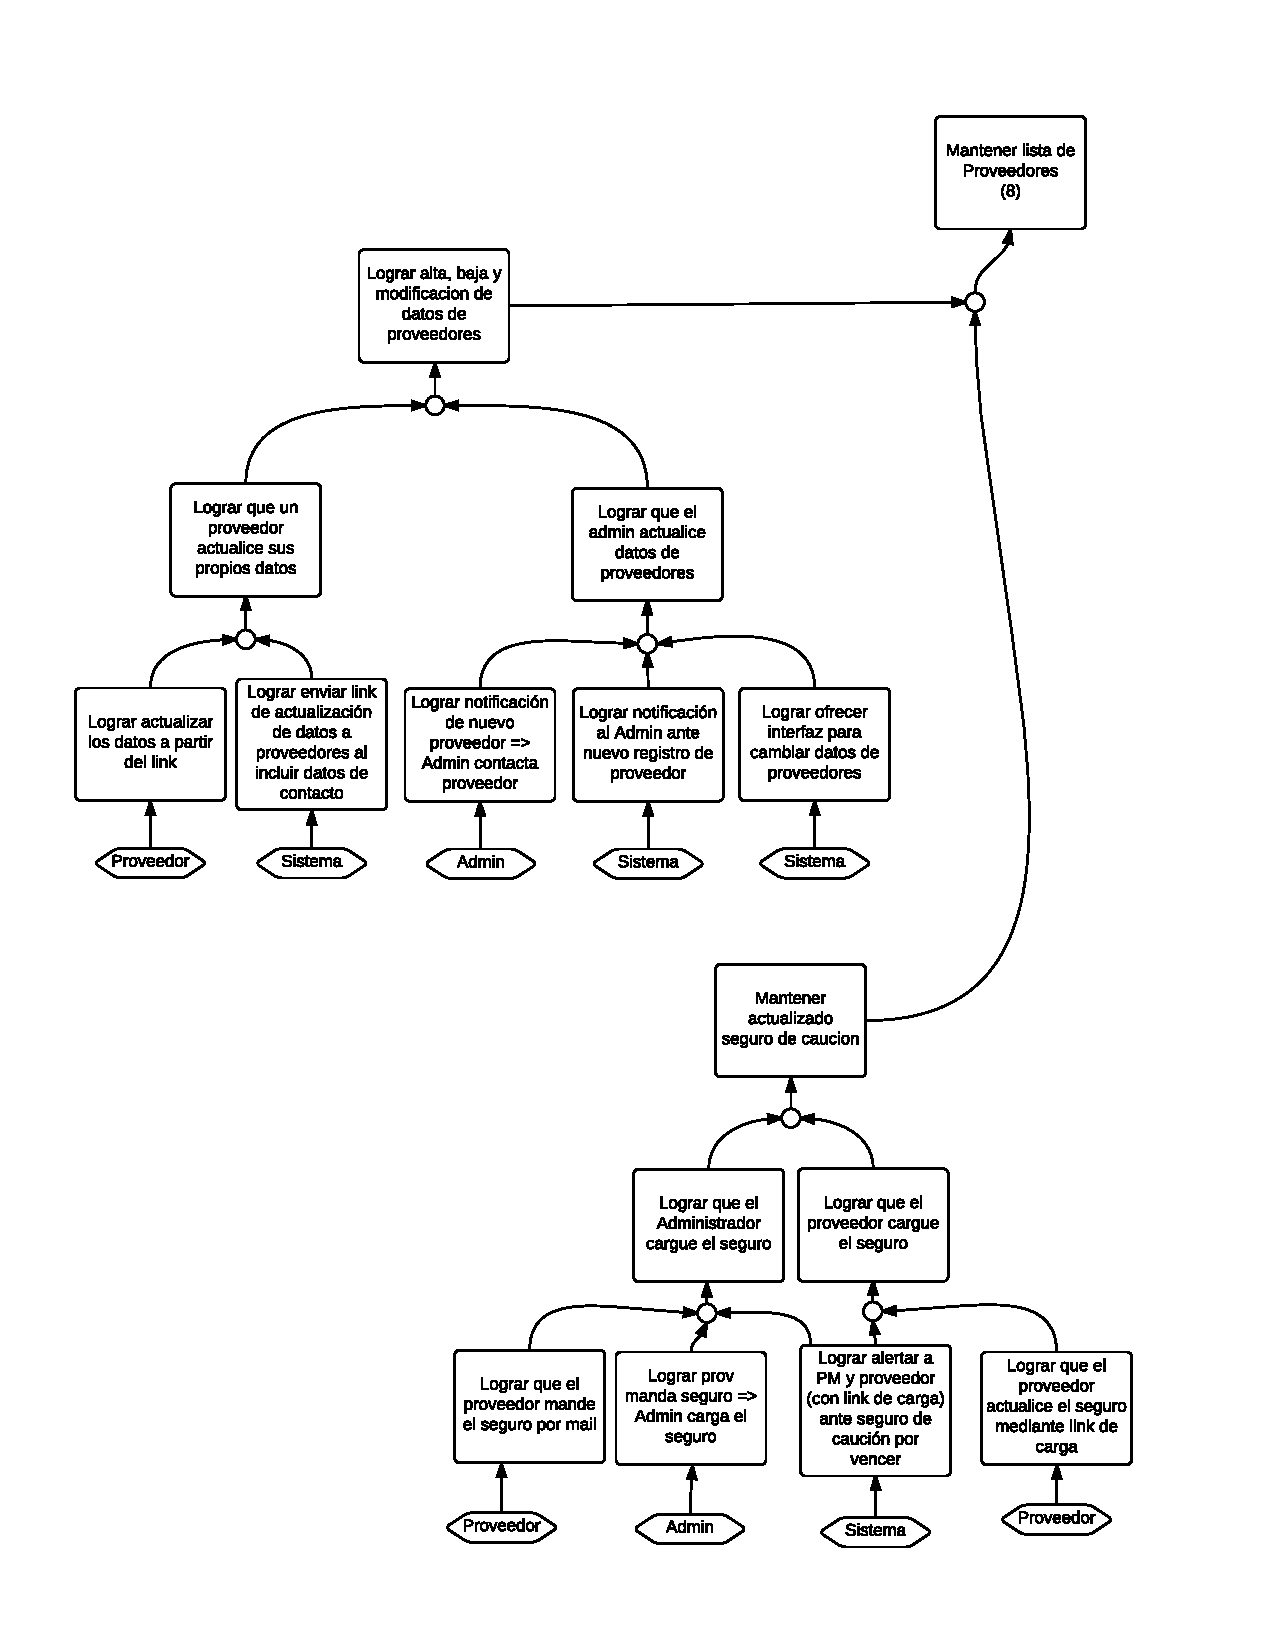
\includegraphics[width=\textwidth, clip=true, trim=15pt 40pt 15pt 40pt]{imagenes/objetivos/objetivos16.pdf}
\end{figure}

\newpage
\subsubsection{Requerimientos de Sistema}
Los requerimientos para esta parte son:
\begin{itemize}
	\item Ofrecer al cliente la opción de cargar un proyecto junto con su información de contacto.
	\item Sobre datos de clientes:
	\begin{itemize}
		\item Ofrecer al PM y Gerente la opción de cargar un proyecto con datos del cliente. %AGREGAR
		\item Ofrecer una forma de visualizar y consultar datos de clientes.
		\item Ofrecer al PM y Gerente la posibilidad de dar de alta, de baja o modificar datos de clientes.
	\end{itemize}
	\item Sobre datos de proveedores:
	\begin{itemize}
		\item Enviar un link a proveedores para completar su información dada la entrada de información de contacto.
		\item Notificar Admin ante el alta de un proveedor (datos de contacto).
		\item Permitir al Admin modificar datos de proveedores.
		\item Notificar Proveedor y Admin ante el próximo vencimiento de un seguro de caución.
		\item Enviar un link de carga de seguro de caución al proveedor, junto con la alerta.
		\item Permitir al Admin cargar un seguro de caución.
	\end{itemize}
\end{itemize}

\subsection{Feedback}
\begin{figure}[H]
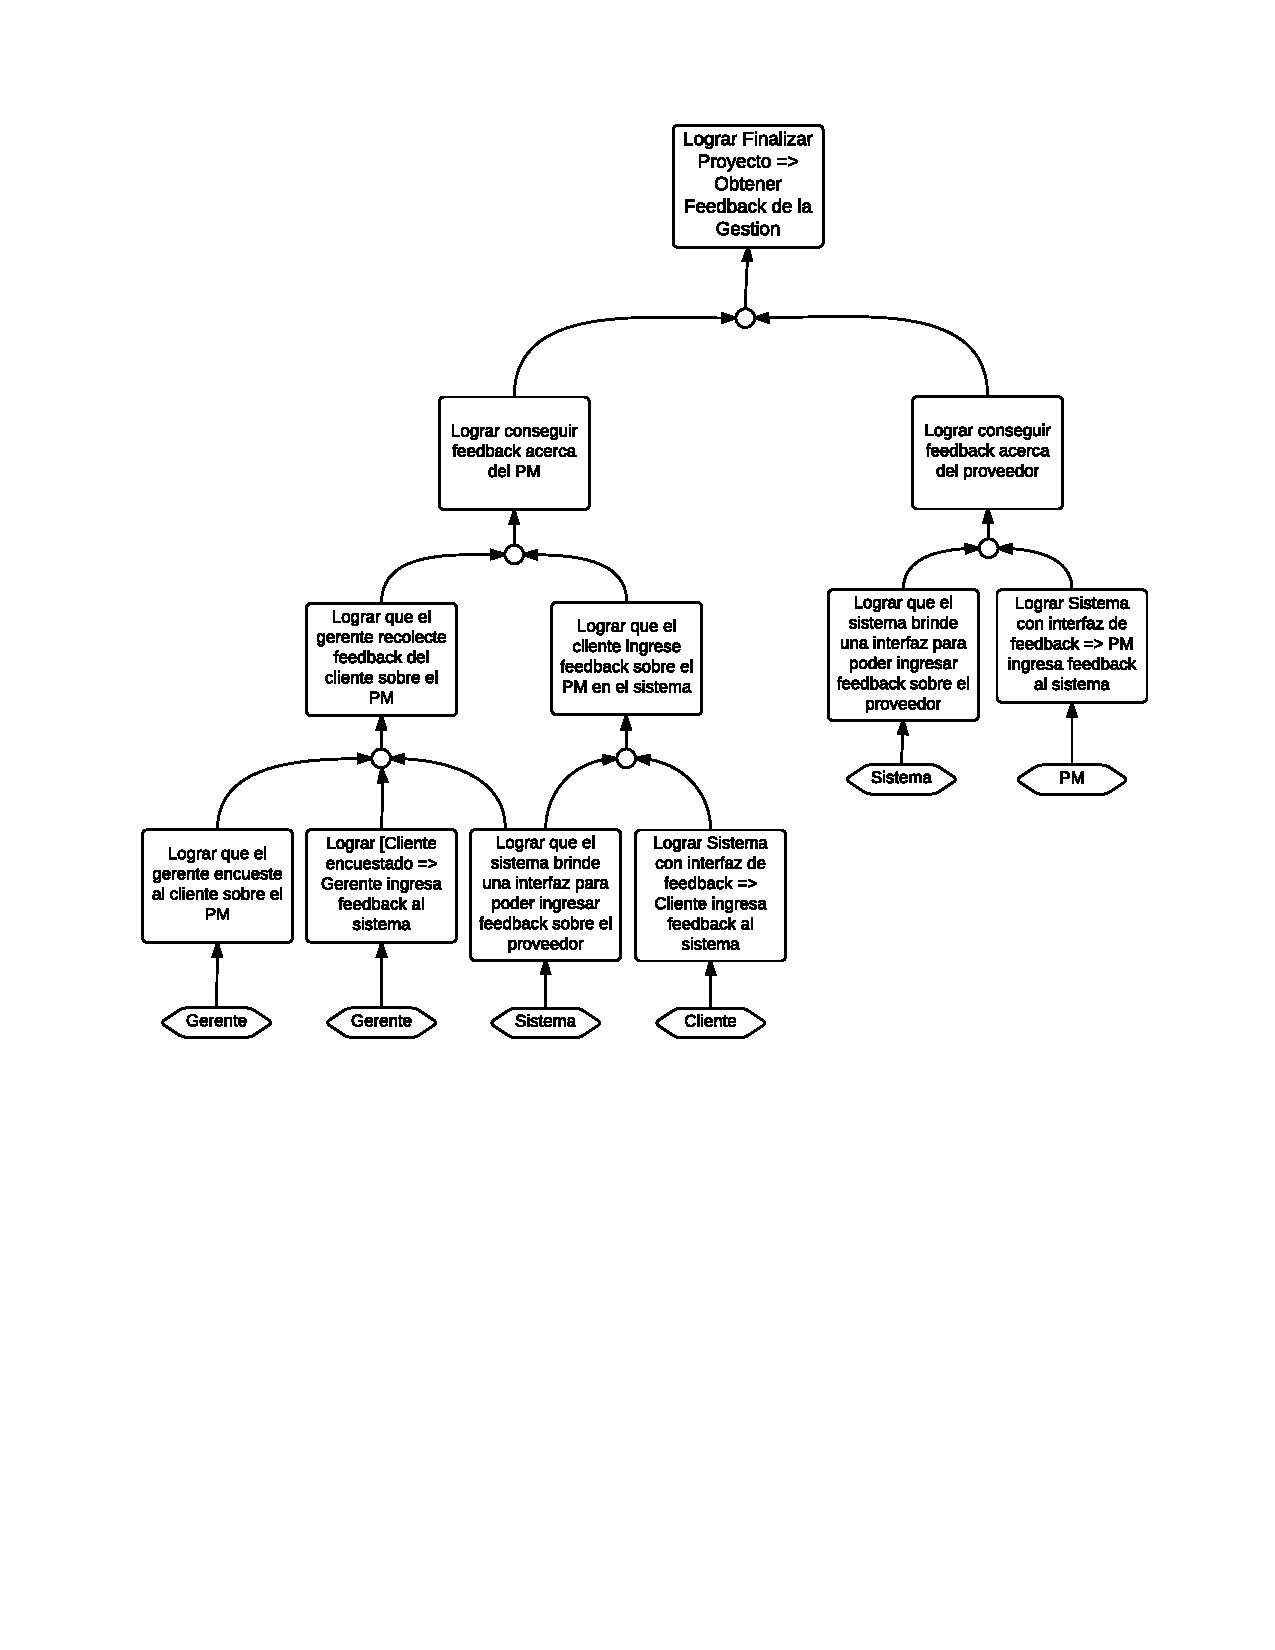
\includegraphics[width=\textwidth, clip=true, trim=15pt 0pt 15pt 0pt]{imagenes/objetivos/objetivos17.pdf}
\end{figure}
